\documentclass[11pt]{book}
\usepackage[utf8]{inputenc}
\usepackage{amsfonts, amssymb, amsmath, amsthm, booktabs, hyperref, pgfplots, tikz, xcolor, mathrsfs, multicol, array}
\usepackage{makeidx}

\theoremstyle{definition}\newtheorem{definition}[subsection]{Definition}
\theoremstyle{definition}\newtheorem{example}[subsection]{Example}
\theoremstyle{definition}\newtheorem{notation}[subsection]{Notation}
\theoremstyle{definition}\newtheorem{remark}[subsection]{Remark}
\theoremstyle{theorem}\newtheorem{theorem}[subsection]{Theorem}
\theoremstyle{theorem}\newtheorem{lemma}[subsection]{Lemma}
\theoremstyle{theorem}\newtheorem{proposition}[subsection]{Proposition}
\theoremstyle{theorem}\newtheorem{corollary}[subsection]{Corollary}

\newcommand{\K}{\mathbb{K}}
\newcommand{\C}{\mathbb{C}}
\newcommand{\CC}{\mathcal{C}}
\newcommand{\R}{\mathbb{R}}
\newcommand{\RR}{\mathcal{R}}
\newcommand{\Q}{\mathbb{Q}}
\newcommand{\Z}{\mathbb{Z}}
\newcommand{\N}{\mathbb{N}}
\newcommand{\F}{\mathbb{F}}
\renewcommand{\H}{\mathbb{H}}
\newcommand{\M}{\mathcal{M}}
\newcommand{\T}{\mathbb{T}}
\newcommand{\TT}{\mathcal{T}}
\DeclareMathOperator{\Char}{char}
\newcommand{\teq}{\trianglelefteq}

\title{\textbf{MATH 3022: Algebra II \\ (Ring Theory)}}
\author{Joe Tran}
\date{\today}

\newcolumntype{P}[1]{>{\centering\arraybackslash}p{#1}}

\makeindex

\begin{document}

\maketitle

\tableofcontents

\chapter{Introduction to Ring Theory}

In MATH 3021 Algebra I, we have studied sets with a single binary operation satisfying certain axioms, but now we are interested in working with sets that have two binary operations. For example, one of the most natural algebraic structures to study is the integers with the operations of addition and multiplication. These operations are related to one another by the distributive property. If we consider a set with two such related binary operations satisfying certain axioms, we have an algebraic structure called a ring. In a ring, we add and multiply elements such as real numbers, complex numbers, matrices, and functions.

\section{Rings}

\begin{definition}\label{definition:1.1.1}\index{ring}
    A nonempty set $R$ is called a \emph{ring} if it has two closed binary operations, addition and multiplication that satisfy the following conditions:
    \begin{enumerate}
        \item For all $a, b \in R$, $a + b = b + a$
        \item For all $a, b, c \in R$, $(a + b) + c = a + (b + c)$
        \item There exists an element $0 \in R$ such that $a + 0 = a$ for all $a \in R$.
        \item For every element $a \in R$, there exists an element $-a \in R$ such that $a + (-a) = 0$.
        \item For all $a, b, c \in R$, $(ab)c = a(bc)$.
        \item For all $a, b, c \in R$, $a(b + c) = ab + ac$ and $(a + b)c = ac + bc$.
    \end{enumerate}
    We denote that $R$ is a ring with addition and multiplication by $(R, +, \cdot)$.
\end{definition}

The last condition is called the \emph{distributive axiom}\index{distributive axiom}, and it relates the binary operations of both addition and multiplication. The axioms (1) to (4) require that a ring needs to be an abelian group under addition, so we could have also defined a ring to be an abelian group $(R, +)$, together with a second binary operation satisfying the fifth and sixth conditions given above. \index{group} \index{abelian} \index{binary operation}

\begin{definition}\label{definition:1.1.2} \index{identity}
    If there exists an element $1 \in R$ such that $1 \neq 0$ and $1a = a1 = a$ for every $a \in R$, then $R$ is a ring with \emph{identity}.
\end{definition}

\begin{definition}\label{definition:1.1.3} \index{commutative ring}
    A ring for which $ab = ba$ for all $a, b \in R$ is called a \emph{commutative ring}.
\end{definition}

\begin{definition}\label{definition:1.1.4}\index{integral domain}
    A commutative ring $R$ with identity is called an \emph{integral domain} if for every $a, b \in R$ such that $ab = 0$, either $a = 0$ or $b = 0$.
\end{definition}

\begin{definition}\label{definition:1.1.5}\index{division ring}
    A \emph{division ring} $R$ with an identity in which every nonzero element $R$ is a unit, i.e. for each $a \in R$ with $a \neq 0$, there exists a unique $a^{-1}$ such that $a^{-1} a = aa^{-1} = 1$.
\end{definition}

\begin{definition}\label{definition:1.1.6}\index{field}
    A commutative division ring is called a \emph{field}.
\end{definition}

Below shows the relationship among rings, integral domains, division rings, and fields.
\begin{center}
    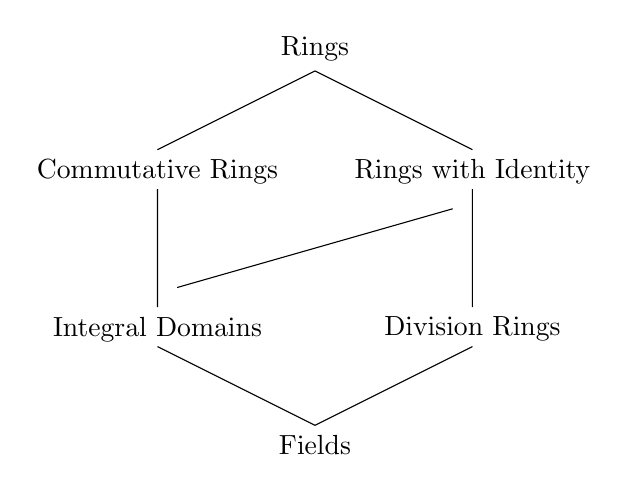
\begin{tikzpicture}
        \node [above] at (0, 0) {Rings};
        \draw (0, 0)--(-2, -1) (0, 0)--(2, -1) node [below] at (-2, -1) {Commutative Rings} node [below] at (2, -1) {Rings with Identity};
        \draw (-2, -1.5)--(-2, -3) (2, -1.5)--(2, -3) node [below] at (-2, -3) {Integral Domains} node [below] at (2, -3) {Division Rings} (-1.75, -2.75)--(1.75, -1.75);
        \draw (-2, -3.5)--(0, -4.5)--(2, -3.5);
        \node [below] at (0, -4.5) {Fields};
    \end{tikzpicture}
\end{center}

\begin{example}\label{example:1.1.7}\index{integer}
    As we have mentioned, the integers form a ring. In fact, $\Z$ is an integral domain. Indeed, if $ab = 0$ for $a, b \in \Z$, then either $a = 0$ or $b = 0$. However, $\Z$ is not a field. That is, there is no such integer that is the multiplicative inverse of 2, since $\frac{1}{2}$ is not an integer. The only integers with multiplicative inverses are 1 and $-1$.
\end{example}

\begin{example}\label{example:1.1.8}\index{addition} \index{multiplication} \index{rational numbers} \index{real numbers} \index{complex numbers}
    Under the ordinary operations of addition and multiplication, all of these familiar number systems are rings: The rationals $\Q$, the real numbers $\R$, and the complex numbers $\C$ are fields.
\end{example}

\begin{notation}\label{notation:1.1.9}
    Whenever we are working with real numbers or complex numbers, we will denote $\K$ to be either the real numbers $\R$ or the complex numbers $\C$. That is, $\K = \R$ or $\K = \C$.
\end{notation}

\begin{notation}\label{notation:1.1.10}
    Whenever we are working with fields, we will denote it by $\F$. For example, $\F = \Q$, $\F = \R$ and $\F = \C$ are all fields.
\end{notation}

\begin{example}\label{example:1.1.11} \index{integer modulo $n$} \index{addition modulo $n$} \index{multiplication modulo $n$}
    Recall that $\Z_n = \{0, 1, 2,..., n - 1\}$ is the \emph{integer modulo $n$} and back in MATH 3021, we have defined the operations $+_n$ and $\cdot_n$, where
    \begin{equation*}
        a +_n b := a + b \pmod n
    \end{equation*}
    and
    \begin{equation*}
        a \cdot_n b := a \cdot b \pmod n
    \end{equation*}
    
    We can define the product of two elements $a, b \in \Z_n$ by $a \cdot_n b$. This product make the abelian group into a ring. Indeed, $\Z_n$ is a commutative ring.

    However, $\Z_n$ fails to be an integral domain. For example, consider $3, 4 \in \Z_{12}$. Then $3 \cdot_{12} 4 = 0$ then we see that the product of two nonzero elements in the ring can be equal to zero.
\end{example}

\begin{definition}\label{definition:1.1.12} \index{zero divisor}
    A nonzero element $a$ in a commutative ring $R$ is called a \emph{zero divisor} if there exists a nonzero element $b \in R$ such that $ab = 0$.
\end{definition}

\begin{example}\label{example:1.1.13}
    In Example \ref{example:1.1.11}, we have that 3 and 4 are zero divisors of $\Z_{12}$.
\end{example}

\begin{notation}\label{notation:1.1.14}\index{set of all continuous functions} \index{set of all continuous functions from $X$ to $Y$}
    We denote the set of all continuous functions from $[a, b]$ to $\K$ by $\CC([a, b])$ and for arbitrary domain and range, we denote it by $\CC(X, Y)$. That is,
    \begin{equation*}
        \CC([a, b]) = \{\text{all continuous functions $f : [a, b] \to \K$}\}
    \end{equation*}
    and
    \begin{equation*}
        \CC(X, Y) = \{\text{all continuous functions $f : X \to Y$}\}
    \end{equation*}
\end{notation}

\begin{example}\label{example:1.1.15}
    $\CC([a, b])$ is a commutative ring. Indeed, we can add or multiply two functions by adding or multiplying the values of the functions. Let $f, g \in \CC([a, b])$ be functions defined by $f(x) = x^2$ and $g(x) = \cos(x)$. Then $(f + g)(x) = f(x) + g(x) = x^2 + \cos(x) \in \CC([a, b])$ and $(fg)(x) = f(x)g(x) = x^2\cos(x) \in \CC([a, b])$.
\end{example}

\begin{notation}\label{notation:1.1.16}\index{set of all $n \times n$ matrices}
    We denote the set of $n \times n$ matrices with $\K$-entries by $\M_n(\K)$. That is,
    \begin{equation*}
        \M_n(\K) = \{\text{all $n \times n$ matrices with $\K$-entries}\}
    \end{equation*}
\end{notation}

\begin{example}\label{example:1.1.17}
    The $n \times n$ with entries $\K = \R$ form a ring under the usual operations of matrix addition and multiplication. However, this ring is noncommuative, since it is usually the case that $AB = BA$. Also, note that we can have $AB = 0$ whenever neither $A$ nor $B$ is zero.
\end{example}

\begin{example}\label{example:1.1.18}
    Let us denote the following matrices
    \begin{equation*}
        1 = \begin{bmatrix}
            1 & 0 \\ 0 & 1 
        \end{bmatrix} \quad
        \mathbf{i} = \begin{bmatrix}
            0 & 1 \\ - 1 & 0
        \end{bmatrix} \quad
        \mathbf{j} = \begin{bmatrix}
            0 & i \\ i & 0 
        \end{bmatrix} \quad
        \mathbf{k} = \begin{bmatrix}
            i & 0 \\ 0 & -i
        \end{bmatrix}
    \end{equation*}
    where $i^2 = -1$. These elements satisfy the following conditions:
    \begin{itemize}
        \item $\mathbf{i}^2 = \mathbf{j}^2 = \mathbf{k}^2 = -1$
        \item $\mathbf{ij} = \mathbf{k}$
        \item $\mathbf{jk} = \mathbf{i}$
        \item $\mathbf{ki} = \mathbf{j}$
        \item $\mathbf{ji} = -\mathbf{k}$
        \item $\mathbf{kj} = -\mathbf{i}$
        \item $\mathbf{ik} = -\mathbf{j}$
    \end{itemize}
\end{example}

\begin{notation}\label{notation:1.1.19}\index{ring of quaternions}
    Let $\H$ denote the elements of the form $a + \mathbf{i}b + \mathbf{j}c + \mathbf{k}d$, where $a, b, c, d \in \R$. Equivalently, we can say that
    \begin{equation*}
        \H = \left\{\begin{bmatrix} \alpha & \beta \\ -\overline{\beta} & \overline{\alpha} \end{bmatrix} : \alpha = a + id, \beta = b + ic \in \C\right\}
    \end{equation*}
\end{notation}

We can define addition and multiplication on $\H$ either by usual matrix operations or in terms of the generators 1, $\mathbf{i}$, $\mathbf{j}$ and $\mathbf{k}$. Indeed,
\begin{align*}
    &(a_1 + b_1\mathbf{i} + c_1\mathbf{j} + d_1\mathbf{k}) + (a_2 + b_2\mathbf{i} + c_2\mathbf{j} + d_2\mathbf{k}) \\
    &= (a_1 + a_2) + (b_1 + b_2)\mathbf{i} + (c_1 + c_2)\mathbf{j} + (d_1 + d_2)\mathbf{k}
\end{align*}
and also
\begin{equation*}
    (a_1 + b_1\mathbf{i} + c_1\mathbf{j} + d_1\mathbf{k})(a_2 + b_2\mathbf{i} + c_2\mathbf{j} + d_2\mathbf{k}) = \alpha + \beta\mathbf{i} + \gamma\mathbf{j} + \delta\mathbf{k}
\end{equation*}
where
\begin{align*}
    \alpha &= a_1a_2 - b_1b_2 - c_1c_2 - d_1d_2 \\
    \beta &= a_1b_2 + a_2b_1 + c_1d_2 - d_1c_2 \\
    \gamma &= a_1c_2 - b_1d_2 + c_1a_2 + d_1b_2 \\
    \delta &= a_1d_2 + b_1c_2 - c_1b_2 + d_1a_2
\end{align*}

After having a look at plenty of examples of types of rings, let us prove the following properties about rings.

\begin{proposition}\label{proposition:1.1.20}
    Let $R$ be a ring and let $a, b \in R$. Then the following hold
    \begin{enumerate}
        \item $a0 = 0a = 0$
        \item $a(-b) = (-a)b = -ab$
        \item $(-a)(-b) = ab$
    \end{enumerate}
\end{proposition}

\begin{proof}
    To see that (1) is true, note that
    \begin{equation*}
        a0 = a(0 + 0) = a0 + a0
    \end{equation*}
    and therefore, $a0 = 0$. Similarly, we also have that $0a = 0$.

    To see that (2) is true, observe that
    \begin{equation*}
        ab + a(-b) = a(b - b) = a0 = 0
    \end{equation*}
    and therefore, $a(-b) = -ab$. Similarly, we also have that $(-a)b = 0$.

    Note that (3) follows from (2) since
    \begin{equation*}
        (-a)(-b) = -(a(-b)) = -(-ab) = ab
    \end{equation*}
\end{proof}

Just as we have subgroups of groups, we have an analogous class of substructures for rings.

\begin{definition}\label{definition:1.1.21}\index{subring}
    A \emph{subring} $S$ of a ring $R$ is a subset $S$ of $R$ such that $S$ is also a ring under the inherited operations from $R$. We denote $S$ is a subring of $R$ as $S \leq R$.
\end{definition}

The following proposition gives us some easy criteria for determining whether or not a subset of a ring is a subring.

\begin{proposition}\label{proposition:1.1.22}
    Let $R$ be a ring and $S \subset R$. Then $S \leq R$ if and only if the following conditions are satisfied:
    \begin{enumerate}
        \item $S \neq \emptyset$.
        \item If $r, s \in S$, $rs \in S$.
        \item If $r, s \in S$, $r - s \in S$.
    \end{enumerate}
\end{proposition}

\begin{proof}
    Assume that $S \leq R$. We need to show that the three conditions hold. Note that because $S$ is a subring of $R$, then $S$ is also a ring, so it cannot be empty. To see that the second and third conditions hold, note that since $S$ is a subring of $R$, the operations are preserved.

    Conversely, if the three conditions hold, we must show that $S$ is a subring under the same operations as $R$. But these conditions are satisfied because of the axioms we have defined for a ring.
\end{proof}

Just like with groups, the following is an immediate consequence of Proposition \ref{proposition:1.1.22}.

\begin{corollary}\label{corollary:1.1.21}
    Let $R$ be a ring with identity and suppose $S \leq R$ if and only if $S \neq \emptyset$ and whenever $r, s, t \in S$, then $r - st \in S$.
\end{corollary}

%\begin{proof}
%    Assume that $S \leq R$. We want to show that $r - st \in S$ whenever $r, s, t \in S$. Since $r, s, t \in S$, then $r - s \in S$ and $st \in S$. Because the closure of the operation, $r - st \in S$.

%    Conversely, suppose that $S \subset R$ such that $S \neq \emptyset$ and $r - st \in S$ whenever $r, s, t \in S$. If $s, t \in S$, then $-s \in S$, and so $0 - (-s)t = st \in S$ and if $r, s \in S$, then $r - s \cdot 1 = r - s \in S$.
%\end{proof}

\begin{example}\label{example:1.1.22}
    The ring $n\Z$ is a subring of $\Z$. Notice that even though the original ring may have an identity, we do not require that its subring have an identity. We have the following chain of subrings:
    \begin{equation*}
        \Z \subset \Q \subset \R \subset \C
    \end{equation*}
\end{example}

\begin{example}\label{example:1.1.23}\index{set of upper triangular matrices}
    Let $R = \M_2(\R)$ and let $\TT_2(\R)$ denote the set of upper triangular matrices in $R$, i.e.
    \begin{equation*}
        \TT_2(\R) = \left\{\begin{bmatrix} a & b \\ 0 & c \end{bmatrix} : a, b, c \in \R\right\}
    \end{equation*}
    Then $\TT_2(\R) \leq \M_2(\R)$. Indeed, if
    \begin{equation*}
        A = \begin{bmatrix}
            a & b \\ 0 & c
        \end{bmatrix} \quad
        B = \begin{bmatrix}
            d & e \\ 0 & f
        \end{bmatrix} \quad
        C = \begin{bmatrix}
            g & h \\ 0 & k
        \end{bmatrix}
    \end{equation*}
    Then by Corollary \ref{corollary:1.1.21}, $\TT_2(\R) \neq \emptyset$, and
    \begin{align*}
        A - BC &= \begin{bmatrix}
            a & b \\ 0 & c
        \end{bmatrix} - \begin{bmatrix}
            d & e \\ 0 & f
        \end{bmatrix}\begin{bmatrix}
            g & h \\ 0 & k
        \end{bmatrix} = \begin{bmatrix}
            a - dg & b - dh - ek \\
            0 & c - kf
        \end{bmatrix} \in \TT_2(\R)
    \end{align*}
\end{example}

\section{Integral Domains and Fields}

In this section, we will be focusing on two types of rings, namely the integral domain (Definition \ref{definition:1.1.4}) and fields (Definition \ref{definition:1.1.6}). \index{integral domain} \index{field}

\begin{example}\label{example:1.2.1}\index{Gaussian integers}
    If $i^2 = -1$, then the set $\Z[i] = \{m + in : a, b \in \Z\}$ forms a ring known as the Gaussian integers. It can be shown that the Gaussian integers are a subring of the complex numbers, i.e. $\Z[i] \leq \C$ since they are closed under addition and multiplication. Let $\alpha = a + ib$ be a unit in $\Z[i]$. THen $\overline{\alpha} = a - ib$ is also a unit since if $\alpha\beta = 1$, then $\overline{\alpha\beta} = 1$. If $\beta = c + id$, then
    \begin{equation*}
        1 = \alpha\beta\overline{\alpha\beta} = (a^2 + b^2)(c^2 + d^2)
    \end{equation*}
    Therefore, $a^2 + b^2$ must be either 1 or $-1$; or equivalently, $a + ib = \pm 1$, or $a + ib = \pm i$. Therefore, units of this ring are $\pm 1$ and $\pm i$. Furthermore, the Gaussian integers are not a field, but it is an integral domain.
\end{example}

\begin{example}\label{example:1.2.2}
    The set of matrices
    \begin{equation*}
        F = \left\{\begin{bmatrix} 1 & 0 \\ 0 & 1 \end{bmatrix}, \begin{bmatrix} 1 & 1 \\ 1 & 0 \end{bmatrix}, \begin{bmatrix} 0 & 1 \\ 1 & 1 \end{bmatrix}, \begin{bmatrix} 0 & 0 \\ 0 & 0 \end{bmatrix}\right\}
    \end{equation*}
    with entries in $\Z_2$ form a field.
\end{example}

\begin{example}\label{example:1.2.3}
    The set $\Q[\sqrt{2}] = \{a + b\sqrt{2} : a, b \in \Q\}$ is a field. The inverse of $a + b\sqrt{2}$ in $\Q[\sqrt{2}]$ is
    \begin{equation*}
        \frac{a}{a^2 - 2b^2} - \frac{b}{a^2 - 2b^2}\sqrt{2}
    \end{equation*}
\end{example}

We have the following alternative characterization of integral domains.

\begin{proposition}[Cancellation Law]\label{proposition:1.2.4}\index{cancellation law}
    Let $D$ be a commutative ring with identity. Then $D$ is an integral domain if and only if for every nonzero elements $d \in D$ with $da = db$, then $a = b$.
\end{proposition}

\begin{proof}
    Let $D$ be an integral domain. Then $D$ has no zero divisors. Let $da = db$ with $d \neq 0$. Then $d(a - b) = 0$, so $a - b = 0$ and thus $a = b$.

    Conversely, suppose that the cancellation law is possible in $D$. That is, suppose that $da = db$ implies $a = b$. Let $da = 0$. If $d \neq 0$, then $da = d0$, or $a = 0$. Therefore, $d$ cannot be a zero divisor.
\end{proof}

\begin{theorem}[Wedderburn]\label{theorem:1.2.5}\index{Wedderburn}
    Every finite integral domain is a field.
\end{theorem}

\begin{proof}
    Let $D$ be a finite integral domain and $D^*$ denote the nonzero elements of $D$. Then we need to show that every element in $D^*$ has an inverse. Let $a \in D^*$ be arbitrary. Define $\lambda_a : D^* \to D^*$ given by $\lambda_a(d) = ad$. We have seen this map previously when we were talking about Group Theory and Cayley's Theorem. This map also makes sense because if $a \neq 0$ and $d \neq 0$, then $ad \neq 0$. The map $\lambda_a$ is also well defined, since for $d_1, d_2 \in D^*$,
    \begin{equation*}
        ad_1 = \lambda_a(d_1) = \lambda_a(d_2) = ad_2
    \end{equation*}
    which implies $d_1 = d_2$ by the cancellation law (Proposition \ref{proposition:1.2.4}). Since $D^*$ is a finite set, the map $\lambda_a$ must also be onto. Therefore, there exists a $d \in D^*$ such that $\lambda_a(d) = ad = 1$. Therefore, $a$ has a left inverse. Since $D$ is commutative, $d$ must also be a right inverse for $a$. Consequently, $D$ is a field.
\end{proof}

\begin{definition}\label{definition:1.2.6}\index{characteristic of a ring}
    For any nonnegative integer $n$ and any element $r$ in a ring $R$, we write
    \begin{equation*}
        \underbrace{r + r + \cdots + r}_{n \ times} = nr
    \end{equation*}
    We define the \emph{characteristic of a ring} $R$ to be the least positive integer $n$ such that $nr = 0$ for all $r \in R$. If no such integer exists, then the characteristic of $R$ is defined to be 0. We will denote the characteristic of $R$ by $\Char(R)$.
\end{definition}

\begin{example}\label{example:1.2.7}
    For every prime $p$, $\Z_p$ is a field of characteristic $p$. Note that every nonzero element in $\Z_p$ has an inverse, and so $\Z_p$ is a field. If $a$ is any nonzero element in the field, then $pa = 0$, since the order of any nonzero element in the abelian group $\Z_p$ is $p$.
\end{example}

\begin{lemma}\label{lemma:1.2.8}
    Let $R$ be a ring with identity. If $1$ has order $n$, then the characteristic of $R$ is $n$.
\end{lemma}

\begin{proof}
    If 1 has order $n$, then $n$ is the least positive integer such that $n1 = 0$. Thus, for any $r \in R$,
    \begin{equation*}
        nr = n(1r) = (n1)r = 0r = 0
    \end{equation*}
    On the other hand, if no positive $n$ exists such that $n1 = 0$, then the characteristic of $R$ is zero.
\end{proof}

We finish this section off with the following theorem.

\begin{theorem}\label{theorem:1.2.9}
    The characteristic of an integral domain is either prime or zero.
\end{theorem}

\begin{proof}
    Let $D$ be an integral domain and suppose that the characteristic of $D$ is $n$ with $n \neq 0$. If $n$ is not prime, then $n = ab$ where $1 < a < n$ and $1 < b < n$. By Lemma \ref{lemma:1.2.8}, we consider the case when $n1 = 0$. SInce $0 = n1 = (ab)1 = (a1)(b1)$ and there are no zero divisors in $D$, either $a1 = 0$ or $b1 = 0$. Hence, the characteristic of $D$ must be less than $n$, which is a contradiction. Therefore, $n$ must be prime.
\end{proof}

\section{Ring Homomorphisms and Ideals}

Recall that when we were talking about groups, a \emph{homomorphism} is a mapping that preserves the operation of the group. That is, if $(G, *)$ and $(H, \star)$ are groups, then if the mapping $\phi : (G, *) \to (H, \star)$ satisfies
\begin{equation*}
    \phi(x * y) = \phi(x) \star \phi(y)
\end{equation*}
Then $\phi$ is said to be a homomorphism, and when such a homomorphism exists, we say that $(G, *)$ is homomorphic to $(H, \star)$ and denote $(G, *) \simeq (H, \star)$. \index{homomorphism} \index{homomorphic}

Furthermore, recall that if $\phi$ is a homomorphism and also it satisfies the property of being a bijection, then $\phi$ is said to be an \emph{isomorphism}. If such a $\phi$ exists, then we say that the groups $(G, *)$ are isomorphic to $(H, \star)$, i.e. $(G, *) \simeq (H, \star)$. \index{isomorphism} \index{homomorphism}

In this section, we will study the ring homomorphisms and introduce the concept of ideals. From now on, whenever we are working with rings, we will be clear that the notation that we are using is $(R, (+, \cdot))$ to indicate that $R$ is the ring and $(+, \cdot)$ are the two binary operations that are associated to ring, but for shorthand notation we will just say that $R$ is a ring.

\begin{definition}\label{definition:1.3.1}\index{ring homomorphism}\index{ring isomorphism}
    Let $(R, (+, \cdot))$ and $(S, (+, \cdot))$ be rings with the respective binary operations. Then a \emph{ring homomorphism} is a mapping $\phi : R \to S$ that satisfies:
    \begin{align*}
        \begin{cases}
            \phi(x + y) &= \phi(x) + \phi(y) \\
            \phi(x \cdot y) &= \phi(x) \cdot \phi(y)
        \end{cases}
    \end{align*}
    for all $x, y \in R$. Furthermore, if $\phi$ is a bijection, then we say that $\phi$ is a \emph{ring isomorphism}.
\end{definition}

We also introduced the concept of the \emph{kernel} when talking about homomorphisms for, but we also have the concept of the kernel for rings as well.

\begin{definition}\label{definition:1.3.2}\index{ring kernel}
    For any ring homomorphism $\phi : R \to S$, we define the \emph{ring kernel} to be the set
    \begin{equation*}
        \ker(\phi) = \{r \in R : \phi(r) = 0\}
    \end{equation*}
\end{definition}

\begin{example}\label{example:1.3.3}
    For any integer $n \in \Z$, we can define a ring homomorphism $\phi : \Z \to \Z_n$ by $\phi(x) = x \pmod n$. This is a ring homomorphism because for any $x, y \in \Z$,
    \begin{align*}
        \phi(x + y) &= (x + y) \pmod n \\
        &= x \pmod n + y \pmod n \\
        &= \phi(x) + \phi(y)
    \end{align*}
    and
    \begin{align*}
        \phi(x \cdot y) &= (x \cdot y) \pmod n \\
        &= x \pmod n \cdot y \pmod n \\
        &= \phi(x) \cdot \phi(y)
    \end{align*}
    Furthermore, the kernel of $\phi$ is the set
    \begin{equation*}
        \ker(\phi) = \{k \in \Z : \phi(k) = 0\} = n\Z
    \end{equation*}
\end{example}

\begin{example}\label{example:1.3.4}\index{evaluation homomorphism}
    Recall that
    \begin{equation*}
        \CC([a, b]) = \{f : [a, b] \to \R : \text{$f$ is continuous}\}
    \end{equation*}
    For any $x \in [a, b]$, we define a ring homomorphism $\phi_x : \CC([a, b]) \to \R$ given by the mapping $\phi_x(f) = f(x)$. This is a ring homomorphism since
    \begin{align*}
        \phi_x(f + g) = (f + g)(x) = f(x) + g(x) = \phi_x(f) + \phi_x(g)
    \end{align*}
    and
    \begin{equation*}
        \phi_x(fg) = (fg)(x) = f(x)g(x) = \phi_x(f)\phi_x(g)
    \end{equation*}
    Ring homomorphisms of this form are called \emph{evaluation homomorphisms}.
\end{example}

In the next proposition, we will examine some fundamental properties of ring homomorphisms.

\begin{proposition}\label{proposition:1.3.5}
    Let $\phi : R \to S$ be a ring homomorphism.
    \begin{enumerate}
        \item If $R$ is a commutative ring, then $\phi(R)$ is a commutative ring.
        \item $\phi(0) = 0$.
        \item Let $1_R$ and $1_S$ be the identities for $R$ and $S$, respectively. If $\phi$ is onto, then $\phi(1_R) = 1_S$.
        \item If $R$ is a field and $\phi(R) \neq 0$, then $\phi(R)$ is a field.
    \end{enumerate}
\end{proposition}

\begin{proof}
    Let $\phi : R \to S$ be a ring homomorphism, and let $x, y \in R$ be arbitrary. To see that (1) is true, observe that because $R$ is a commutative ring and because $\phi$ is a homomorphism, then $xy = yx$, and thus
    \begin{equation*}
        \phi(x)\phi(y) = \phi(xy) = \phi(yx) = \phi(y)\phi(x)
    \end{equation*}
    Therefore, $\phi(R)$ is a commutative ring.

    To see that (2) is true, let $x \in R$ be arbitrary. Then
    \begin{equation*}
        0 \cdot \phi(0) = 0 = \phi(0 \cdot 0) = \phi(0) \phi(0)
    \end{equation*}
    Then by the cancellation law, $\phi(0) = 0$.

    To see that (3) is true, assume that $1_R$ and $1_S$ are identities for $R$ and $S$, respectively. Then
    \begin{equation*}
        1_S\phi(1_R) = \phi(1_R) = \phi(1_R \cdot 1_R) = \phi(1_R)\phi(1_R)
    \end{equation*}
    Then by the cancellation law, $\phi(1_R) = 1_S$.

    To see that (4) is true, let $x \in R$ be a nonzero element such that $\phi(x) \neq 0$. Then because $R$ is a field and $x \neq 0$, then there exists an $x^{-1} \in R$ such that $1_R = x \cdot x^{-1} = x^{-1} \cdot x$. Then observe that because $\phi$ is a homomorphism,
    \begin{equation*}
        \phi(x) \cdot \phi(x^{-1}) = \phi(x) \cdot [\phi(x)]^{-1} = 1_S
    \end{equation*}
    Therefore, $\phi(R)$ is also a field.
\end{proof}

In group theory, we found that normal subgroups play a special role. These subgroups have nice characteristics that make them more interesting to study than arbitrary subgroups. In ring theory, the objects corresponding to normal subgroups are a special class of subrings called ideals. \index{ideal}

\begin{definition}\label{definition:1.3.6}
    An \emph{ideal} in a ring $R$ is a subring $I \leq R$ such that if $a \in I$ and $r \in R$, then $ar, ra \in I$, i.e. $rI \in I$ and $Ir \subset I$ for all $r \in R$. We denote that $I$ is an ideal of $R$ as $I \trianglelefteq R$.
\end{definition}

\begin{example}\label{example:1.3.7}\index{trivial ideal}
    Every ring has at least two ideals, namely the \emph{trivial ideals} $\{0\}$ and $R$.
\end{example}

Let $R$ be a ring with identity and suppose that $I \teq R$ such that $1 \in I$. Since for any $r \in R$, $r1 = r \in I$, by the definition of an ideal, then $I = R$.

\begin{example}\label{example:1.3.8}\index{principal ideal}
    If $a$ is any element in a commutative ring $R$ with identity, then the set
    \begin{equation*}
        \langle{a}\rangle = \{ar : r \in R\}
    \end{equation*}
    is an ideal of $R$. Indeed, $\langle{a}\rangle$ is nonempty since both $0 = a0$ and $a = a1$ are in $\langle{a}\rangle$. The sum of two elements in $\langle{a}\rangle$ is in $\langle{a}\rangle$ since $ar + ar' = a(r + r')$. The inverse of $ar$ is $-ar = a(-r) \in \langle{a}\rangle$. Finally, if we multiply an element $ar \in \langle{a}\rangle$ by an arbitrary element $s \in R$, we have $s(ar) = a(sr)$. Therefore, $\langle{a}\rangle$ satisfies the definition of an ideal.

    If $R$ is a commutative ring with identity, then an ideal of the form $\langle{a}\rangle = \{ar : r \in R\}$ is called a \emph{principal ideal}.
\end{example} 

\begin{theorem}\label{theorem:1.3.9}
    Every ideal in the ring of integers $\Z$ is a principal ideal.
\end{theorem}

\begin{proof}
    The zero ideal $\{0\}$ is a principal ideal since $\langle{0}\rangle = \{0\}$. If $I$ is any nonzero ideal in $\Z$, then $I$ must contain some positive integer $m$. There exists a least positive integer $n$ in $I$, by the Well-Ordering Principal. Now let $a \in I$. By the division algorithm, there exists $q, r$ such that
    \begin{equation*}
        a = nq + r
    \end{equation*}
    where $0 \leq r < n$. This equation suggests that $r = a - nq \in I$, but $r = 0$ since $n$ is the least positive element in $I$, so $a = nq$, and thus, $I = \langle{n}\rangle$, as required.
\end{proof}

\begin{example}\label{example:1.3.10}
    The set $n\Z$ is ideal in the ring of integers. If $na \in n\Z$ and $b \in \Z$, then $nab \in n\Z$. In fact, by Theorem \ref{theorem:1.3.9}, these are the only ideals of $\Z$.
\end{example}

\begin{proposition}\label{proposition:1.3.11}
    The kernel of any ring homomorphism $\phi : R \to S$ is an ideal in $R$.
\end{proposition}

\begin{proof}
    We know from group theory that $\ker(\phi)$ is an additive subgroup of $R$. Suppose that $r \in R$ and $a \in \ker(\phi)$. Then we must show that $ar$ and $ra$ are in $\ker(\phi)$. However,
    \begin{equation*}
        \phi(ar) = \phi(a)\phi(r) = 0\phi(r) = 0
    \end{equation*}
    and similarly,
    \begin{equation*}
        \phi(ra) = \phi(r)\phi(a) = \phi(r)0 = 0
    \end{equation*}
    as desired.
\end{proof}

\begin{remark}\label{remark:1.3.12}\index{two-sided ideals}\index{one-sided ideals}\index{left ideals}\index{right ideals}
    In our definition of an ideal, we have required that $rI \subset I$ and $Ir \subset I$ for all $r \in R$. Such ideals are sometimes referred to as \emph{two-sided ideals}. We can also consider \emph{one-sided ideals}; that is, we may require only that either $rI \subset I$ or $Ir \subset I$ for $r \in R$ hold, but not both. Such ideals are called \emph{left ideals} and \emph{right ideals}, respectively. Of course, in a commutative ring, any ideal must be two-sided.
\end{remark}

\begin{theorem}\label{theorem:1.3.13}
    Let $I \teq R$. The factor group $R/I$ is a ring with multiplication defined by
    \begin{equation*}
        (r + I)(s + I) = rs + I
    \end{equation*}
\end{theorem} 

\begin{proof}
    We already know that $R/I$ is an abelian group under addition. Let $r + I$ and $s + I$ be in $R/I$. We need to show that $(r + I)(s + I) = rs + I$ is independent of the choice of coset. That is, if $r' \in r + I$ and $s' \in s + I$, then $r's' \in rs + I$. Since $r' \in r + I$, then there exists an $a \in I$ such that $r' = r + a$. Similarly, there exists a $b \in I$ such that $s' = s + b$. Then observe
    \begin{equation*}
        r's' = (r + a)(s + b) = rs + as + rb + ab
    \end{equation*} 
    and $as + rb + ab \in I$, since $I$ is an ideal. Consequently, we obtain that $r's' \in rs + I$.
\end{proof}

The ring $R/I$ in Theorem \ref{theorem:1.3.13} is called the \emph{factor ring} or \emph{quotient ring}. Just as with group homomorphisms and normal subgroups, there is a relationship between ring homomorphisms and ideals. \index{factor ring} \index{quotient ring}

\begin{theorem}\label{theorem:1.3.14}
    Let $I \teq R$. The map $\phi : R \to R/I$ defined by $\phi(r) = r + I$ is a surjective ring homomorphism with kernel $I$.
\end{theorem}

\begin{proof}
    Clearly, $\phi$ is a surjective abelian group homomorphism. Finally, it remains to show that $\phi$ works under ring multiplication. If $r, s \in R$, then
    \begin{equation*}
        \phi(r)\phi(s) = (r + I)(s + I) = rs + I = \phi(rs)
    \end{equation*}
    as required.
\end{proof}

The map $\phi : R \to R/I$ is called the \emph{natural homomorphism} or \emph{canonical homomorphism}. In ring theory, we have isomorphism theorems relating ideals and ring homomorphisms similar to the isomorphism theorems for groups that relate normal subgroups and homomorphisms. \index{natural homomorphism}\index{canonical homomorphism}

\begin{theorem}[The First Isomorphism Theorem]\label{theorem:1.3.15}\index{first isomorphism theorem}
    Let $\psi : R \to S$ be a ring homomorphism. Then $\ker(\psi)$ is an ideal of $R$. If $\phi : R \to R/\ker(\psi)$ is the canonical homomorphism, then there exists a unique isomorphism $\eta : R/\ker(\psi) \to \psi(R)$ such that $\psi = \eta\phi$.
\end{theorem}

\begin{proof}
    Let $K = \ker(\phi)$. By the First Isomorphism Theorem for groups, there exists a well-defined group homomorphism $\eta : R/K \to \psi(R)$ defined by $\eta(r + K) = \psi(r)$ for the additive abelian groups $R$ and $R/K$. To show that this is a ring homomorphism, we need only show that $\eta((r + K)(s + K)) = \eta(r + K)\eta(s + K)$. Indeed,
    \begin{align*}
        \eta((r + K)(s + K)) &= \eta(rs + K) \\
        &= \psi(rs) \\
        &= \psi(r)\psi(s) \\
        &= \eta(r + K)\eta(s + K)
    \end{align*}
    as desired.
\end{proof}

\begin{theorem}[The Second Isomorphism Theorem]\label{theorem:1.3.16}\index{second isomorphism theorem}
    Let $R$ be a ring, let $I \leq R$ and $J \teq R$. Then $I \cap J$ is an ideal of $I$, and
    \begin{equation*}
        I/(I \cap J) \simeq (I + J)/J
    \end{equation*}
\end{theorem}

\begin{theorem}[The Third Isomorphism Theorem]\label{theorem:1.3.17}\index{third isomorphism theorem}
    Let $R$ be a ring and $I, J \teq R$ where $J \subset I$. Then
    \begin{equation*}
        R/I \simeq \frac{R/J}{I/J}
    \end{equation*}
\end{theorem}

\begin{theorem}[Correspondence Theorem]\label{theorem:1.3.17}\index{correspondence theorem}
    Let $R$ be a ring and let $I \teq R$. Then $S \mapsto S/I$ is a bijection between $S \leq R$ containing $I$ and $R/I \leq R$. Furthermore, the ideals of $R$ containing $I$  correspond to ideals of $R/I$.
\end{theorem}

\chapter{Polynomials}

Most people are fairly familiar with polynomials by the time they begin to study abstract algebra. When we examine polynomial expressions such as
\begin{equation*}
    p(x) = x^3 - 3x + 2 \quad q(x) = 3x^2 - 6x + 5
\end{equation*}
we have a pretty good idea of what $p(x) + q(x)$ and $p(x)q(x)$ mean. We just add and multiply polynomials as functions, that is,
\begin{align*}
    (p + q)(x) &= p(x) + q(x) \\
    &= (x^3 - 3x + 2) + (3x^2 - 6x + 5) \\
    &= x^3 + 3x^2 - 9x + 7
\end{align*}
and
\begin{align*}
    (pq)(x) &= p(x)q(x) \\
    &= (x^3 - 3x + 2)(3x^2 - 6x + 5) \\
    &= 3x^5- 6x^4 - 4x^3 + 24x^2 - 27x + 10
\end{align*}

In this chapter, we will emphasize the algebraic structure of polynomials by studying polynomial rings. We can prove many results of polynomials by studying polynomial rings. We can prove many results for polynomial rings that are similar to the theorems we proved for integers. Analogues of prime numbers, the division algorithm, and the Euclidean algorithm exist for polynomials.

\section{Polynomial Rings}

Throughout this chapter we shall assume that $R$ is a commutative ring with identity.

\begin{definition}\label{definition:2.1.1}\index{polynomial}\index{polynomial over $R$}\index{indeterminate}
    Any expression of the form
    \begin{equation*}
        f(x) = \sum_{i = 0}^{n} a_ix^i = a_0 + a_1x + a_2x^2 + \cdots + a_nx^n
    \end{equation*}
    where $a_i \in R$ and $a_n \neq 0$, is called the \emph{polynomial over $R$} with \emph{indeterminate} $x$.
\end{definition}

\begin{definition}\label{definition:2.1.2}\index{coefficient}\index{leading coefficient}
    Let $R$ be a ring. For each $0 \leq i \leq n$, $a_i \in R$ is called the \emph{coefficients} of the polynomial $f$, and $a_n \in R$ is called the \emph{leading coefficient}.
\end{definition}

\begin{definition}\label{definition:2.1.3}\index{monic}
    A polynomial is said to be \emph{monic} if the leading coefficient is 1.
\end{definition}

\begin{definition}\label{definition:2.1.4}\index{degree}
    If $n$ is the largest nonnegative number for which $a_n \neq 0$, we say that the \emph{degree of $f$} is $n$, and denote it as $\deg(f) = n$. If no such $n$ exists, i.e. $f$ is the zero polynomial, then the degree of $f$ is said to be $-\infty$.
\end{definition}

\begin{notation}\label{notation:2.1.5}\index{polynomial ring}
    We denote the set of all polynomials with coefficients in a ring $R$ as $R[x]$.
\end{notation}

\begin{definition}\label{definition:2.1.6}\index{equal}
    If $p(x) = \sum_{i = 0}^{n} a_ix^i$ and $q(x) = \sum_{i = 0}^{m} b_ix^m$ are two polynomials in $R[x]$, then we say that $p(x)$ is \emph{equal} to $q(x)$, if $n = m$, and for every $0 \leq i \leq n$, $a_i = b_i$.
\end{definition}

We define polynomial addition and polynomial multiplication over $R$ as follows: Let $p(x)$ and $q(x)$ be polynomials in $R[x]$ given by
\begin{equation*}
    p(x) = \sum_{i = 0}^{n} a_ix^i \quad q(x) = \sum_{i = 0}^{m} b_ix^i
\end{equation*}
Then we define polynomial addition as
\begin{equation*}
    (p + q)(x) = c_0 + c_1x + \cdots + c_kx^k
\end{equation*}
where for each $0 \leq i \leq n$, $c_i = a_i + b_i$. Similarly, we define polynomial multiplication as
\begin{equation*}
    (pq)(x) = c_0 + c_1x + \cdots + c_{m + n}x^{m + n}
\end{equation*}
where for each $0 \leq i \leq n$, $c_i = \sum_{k = 0}^{i} a_kb_{i - k}$. \index{polynomial addition} \index{polynomial multiplication}

\begin{remark}\label{remark:2.1.7}
    Note that in some cases, the coefficients may be zero, except for the leading coefficient.
\end{remark}

\begin{example}\label{example:2.1.8}
    Let $p(x) = 3 + 2x^3$ and $q(x) = 2 - x^2 + 4x^4$ be polynomials in $\Z[x]$. Then by applying polynomial addition and polynomial multiplication over $\Z$, then
    \begin{align*}
        (p + q)(x) &= (3 + 2x^3) + (2 - x^2 + 4x^4) \\
        &= (3 + 2) + (0 + 0)x + (0 - 1)x^2 + (2 + 0)x^3 + (0 + 4)x^4 \\
        &= 5 - x^2 + 2x^3 + 4x^4
    \end{align*}
    and
    \begin{align*}
        (pq)(x) &= (3 + 2x^3)(2 - x^2 + 4x^4) \\
        &= 6 - 3x^2 + 4x^3 + 12x^4 - 2x^5 + 8x^7
    \end{align*}
\end{example}

\begin{example}\label{example:2.1.9}
    Let $p(x) = 3 + 3x^3$ and $q(x) = 4 + 4x^2 + 4x^4$ be polynomials in $\Z_{12}[x]$. Then
    \begin{align*}
        (p + q)(x) &= (3 + 3x^3) + (4 + 4x^2 + 4x^4) \\
        &= 7 + 4x^2 + 3x^3 + 4x^4
    \end{align*}
    and $(pq)(x) = 0$.
\end{example}

\begin{remark}\label{remark:2.1.10}
    In Example \ref{example:2.1.9}, we see that when we multiply the two polynomials $p(x)$ and $q(x)$ together, we end up with the zero polynomial. In this case, we cannot expect $R[x]$ to be an integral domain if $R$ is not an integral domain.
\end{remark}

\begin{proposition}\label{proposition:2.1.11}
    Let $R$ be a commutative ring with identity. Then $R[x]$ is a commutative ring with identity.
\end{proposition}

\begin{proof}
    To show that $R[x]$ is a commutative ring with identity, we first need to show that $R[x]$ is an abelian group under polynomial addition. In this case, $f(x) = 0$ is the additive identity. If $p(x) = \sum_{i = 0}^{n} a_ix^i$ is a polynomial in $R[x]$, then the inverse is simply the additive inverse $-p(x) = \sum_{i = 0}^{n} (-a_i)x^i = -\sum_{i = 0}^{n} a_ix^i$. Showing that $R[x]$ is associative and abelian under addition follow immediately from the definition of polynomial addition and from the fact that $R$ is also abelian and commutative under addition.

    To show that polynomial multiplication is associative, let
    \begin{equation*}
        p(x) = \sum_{i = 0}^{n} a_ix^i \quad q(x) = \sum_{i = 0}^{m} b_ix^i \quad r(x) = \sum_{i = 0}^{\ell} c_ix^i
    \end{equation*}
    Then
    \begin{align*}
        [(pq)r](x) &= \left[\left(\sum_{i = 0}^{m} a_ix^i\right)\left(\sum_{i = 0}^{n} b_ix^i\right)\right]\left(\sum_{i = 0}^{\ell} c_ix^i\right) \\
        &= \left[\sum_{i = 0}^{n + m} \left(\sum_{j = 0}^{i} a_jb_{i - j}\right)x^i\right]\left(\sum_{i = 0}^{\ell} c_ix^i\right) \\
        &= \sum_{i = 0}^{n + m + \ell} \left[\sum_{j = 0}^{i} \left(\sum_{k = 0}^{j} a_k b_{j - k}\right)c_{i - j}\right]x^i \\
        &= \sum_{i = 0}^{n + m + \ell} \left(\sum_{i = j + k + s} a_j b_k c_s\right)x^i \\
        &= \sum_{i = 0}^{n + m + \ell} \left[\sum_{j = 0}^{i} a_j\left(\sum_{k = 0}^{i - j} b_k c_{i - j - k}\right)\right]x^i \\
        &= \left(\sum_{i = 0}^{n} a_ix^i\right)\left[\sum_{i = 0}^{m + \ell} \left(\sum_{j = 0}^{i} b_j c_{i - j}\right)x^i\right] \\
        &= \left(\sum_{i = 0}^{n} a_ix^i\right)\left[\left(\sum_{i = 0}^{m} b_ix^i\right)\left(\sum_{i = 0}^{\ell} c_ix^i\right)\right] \\
        &= [p(qr)](x)
    \end{align*}
    The commutativity and distributive properties of polynomial multiplication are proven in a similar manner.
\end{proof}

\begin{proposition}\label{proposition:2.1.12}
    Let $p(x)$ and $q(x)$ be polynomials in $R[x]$, where $R$ is an integral domain. Then $\deg(p) + \deg(q) = \deg(pq)$. Furthermore, $R[x]$ is an integral domain.
\end{proposition}

\begin{proof}
    Let $p(x)$ and $q(x)$ be two polynomials given by
    \begin{equation*}
        p(x) = \sum_{i = 0}^{n} a_ix^i \quad q(x) = \sum_{i = 0}^{m} b_ix^i
    \end{equation*}
    with $a_n \neq 0$ and $b_m \neq 0$. Then $\deg(p) = n$ and $\deg(q) = m$ respectively. The leading term of $p(x)q(x)$ is $a_mb_nx^{m + n}$, which cannot be zero because $R$ is an integral domain. Therefore, $\deg(pq) = n + m$, and $p(x)q(x) \neq 0$. Since $p(x) \neq 0$ and $q(x) \neq 0$ imply that $p(x)q(x) \neq 0$, we know that $R[x]$ must also be an integral domain.
\end{proof}

Suppose we want to consider polynomials of two or more variables. Let $R$ be a ring and suppose that $x$ and $y$ are indeterminates. Then we denote the polynomial ring over $x$ and $y$ as $(R[x])[y]$. Although it is straightforward, it is also a tedious task to show that $(R[x])[y] \simeq R([y])[x]$. We will denote the ring instead, by $R[x, y]$. The ring $R[x, y]$ is called the \emph{ring of polynomials in two indeterminates $x$ and $y$ with coefficients in $R$}. We can also denote the \emph{ring of polynomials in $n$ indeterminates with coefficients in $R$}, and we denote it by $R[x_1, x_2,..., x_n]$. \index{polynomial ring in two indeterminates} \index{polynomial ring in $n$ indeterminates}

\begin{theorem}\label{theorem:2.1.13}
    Let $R$ be a commutative ring with identity and $\alpha \in R$, then we have a ring homomorphism $\phi_{\alpha} : R[x] \to R$ defined by
    \begin{equation*}
        \phi_{\alpha}(p(x)) = p(\alpha) = a_n\alpha^n + \cdots + a_1\alpha + a_0
    \end{equation*}
    where $p(x) = a_nx^n + \cdots + a_0$. The map $\phi_{\alpha}$ is called the \emph{evaluation homomorphism at $\alpha$}. \index{evaluation homomorphism}
\end{theorem}

\begin{proof}
    To show that $\phi_{\alpha}$ is a ring homomorphism, let $p(x) = \sum_{i = 0}^{n} a_ix^i$ and $q(x) = \sum_{i = 0}^{m} b_ix^i$ be polynomials in $R[x]$. Then it is elementary to see that
    \begin{equation*}
        \phi_{\alpha}(p(x) + q(x)) = \phi_{\alpha}(p(x)) + \phi_{\alpha}(q(x))
    \end{equation*}
    For the multiplication, note that
    \begin{align*}
        \phi_{\alpha}(p(x))\phi_{\alpha}(q(x)) &= p(\alpha)q(\alpha) \\
        &= \left(\sum_{i = 0}^{n} a_i\alpha^i\right)\left(\sum_{i = 0}^{m} b_i\alpha^i\right) \\
        &= \sum_{i = 0}^{n + m} \left(\sum_{k = 0}^{i} a_k b_{i - k}\right) \alpha^i \\
        &= \phi_{\alpha}(p(x)q(x))
    \end{align*}
\end{proof}

\printindex

\end{document}